\documentclass{amsart}
\usepackage{hyperref, tikz}

\begin{document}

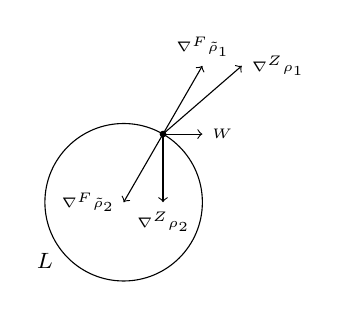
\begin{tikzpicture}
\draw (0,0) circle [radius=1];
\node at (-1,-3/4) {\footnotesize $L$};
\filldraw (1/2,1.73205/2) circle (1pt) coordinate (p);
\path (p)  ++(60:1) coordinate (f1);
\path (p)  ++(60:-1) coordinate (f2);
\draw [->] (p) -- (f1) node[above] {\tiny $\nabla^F \tilde \rho_1$};
\draw[->] (p) -- (f2) node[below,left] {\tiny $\nabla^F \tilde \rho_2$};
\path (f1)  ++(0:1/2) coordinate (z1);
\path (f2)  ++(0:1/2) coordinate (z2);
\draw [->] (p) -- (z1) node[above,right] {\tiny $\nabla^Z \rho_1$};
\draw[->] (p) -- (z2) node[below] {\tiny $\nabla^Z \rho_2$};
\path (p) ++(0:1/2) coordinate (w);
\draw[->] (p) -- (w) node[right] {\tiny $W$};
\end{tikzpicture}

\end{document}